\chapter{Introduction}
In the never-ending quest of advancing wireless communication technology, the use of \ac{mmWave} frequencies has begun with 5G, thus offering future-proof data rates and network capacity due to the large available bandwidth \cite{Intro1, ericsson6g, nokia6g}. However, path loss at \ac{mmWave} frequency is much higher, particularly due to reduced object penetration, thus greatly reducing the effective cell and causing shadowing within \cite{6GWireless, 8373698}. 

Looking toward the future 6G, this shall be addressed by new concepts such as \ac{SRE}s \cite{CNI}. There, metasurfaces shall be used to improve connectivity, among other things, by using their capability to deliberately modify the reflection behavior of an impinging incident wave. There are two kinds of metasurfaces: \ac{IRS} and passive reflectors.
\begin{figure}[H]
	\centering
	\subfloat[mmWave communication in a nutshell with RX1 in LOS has well connectivity, and RX2 in NLOS condition has a poor connection.]{
		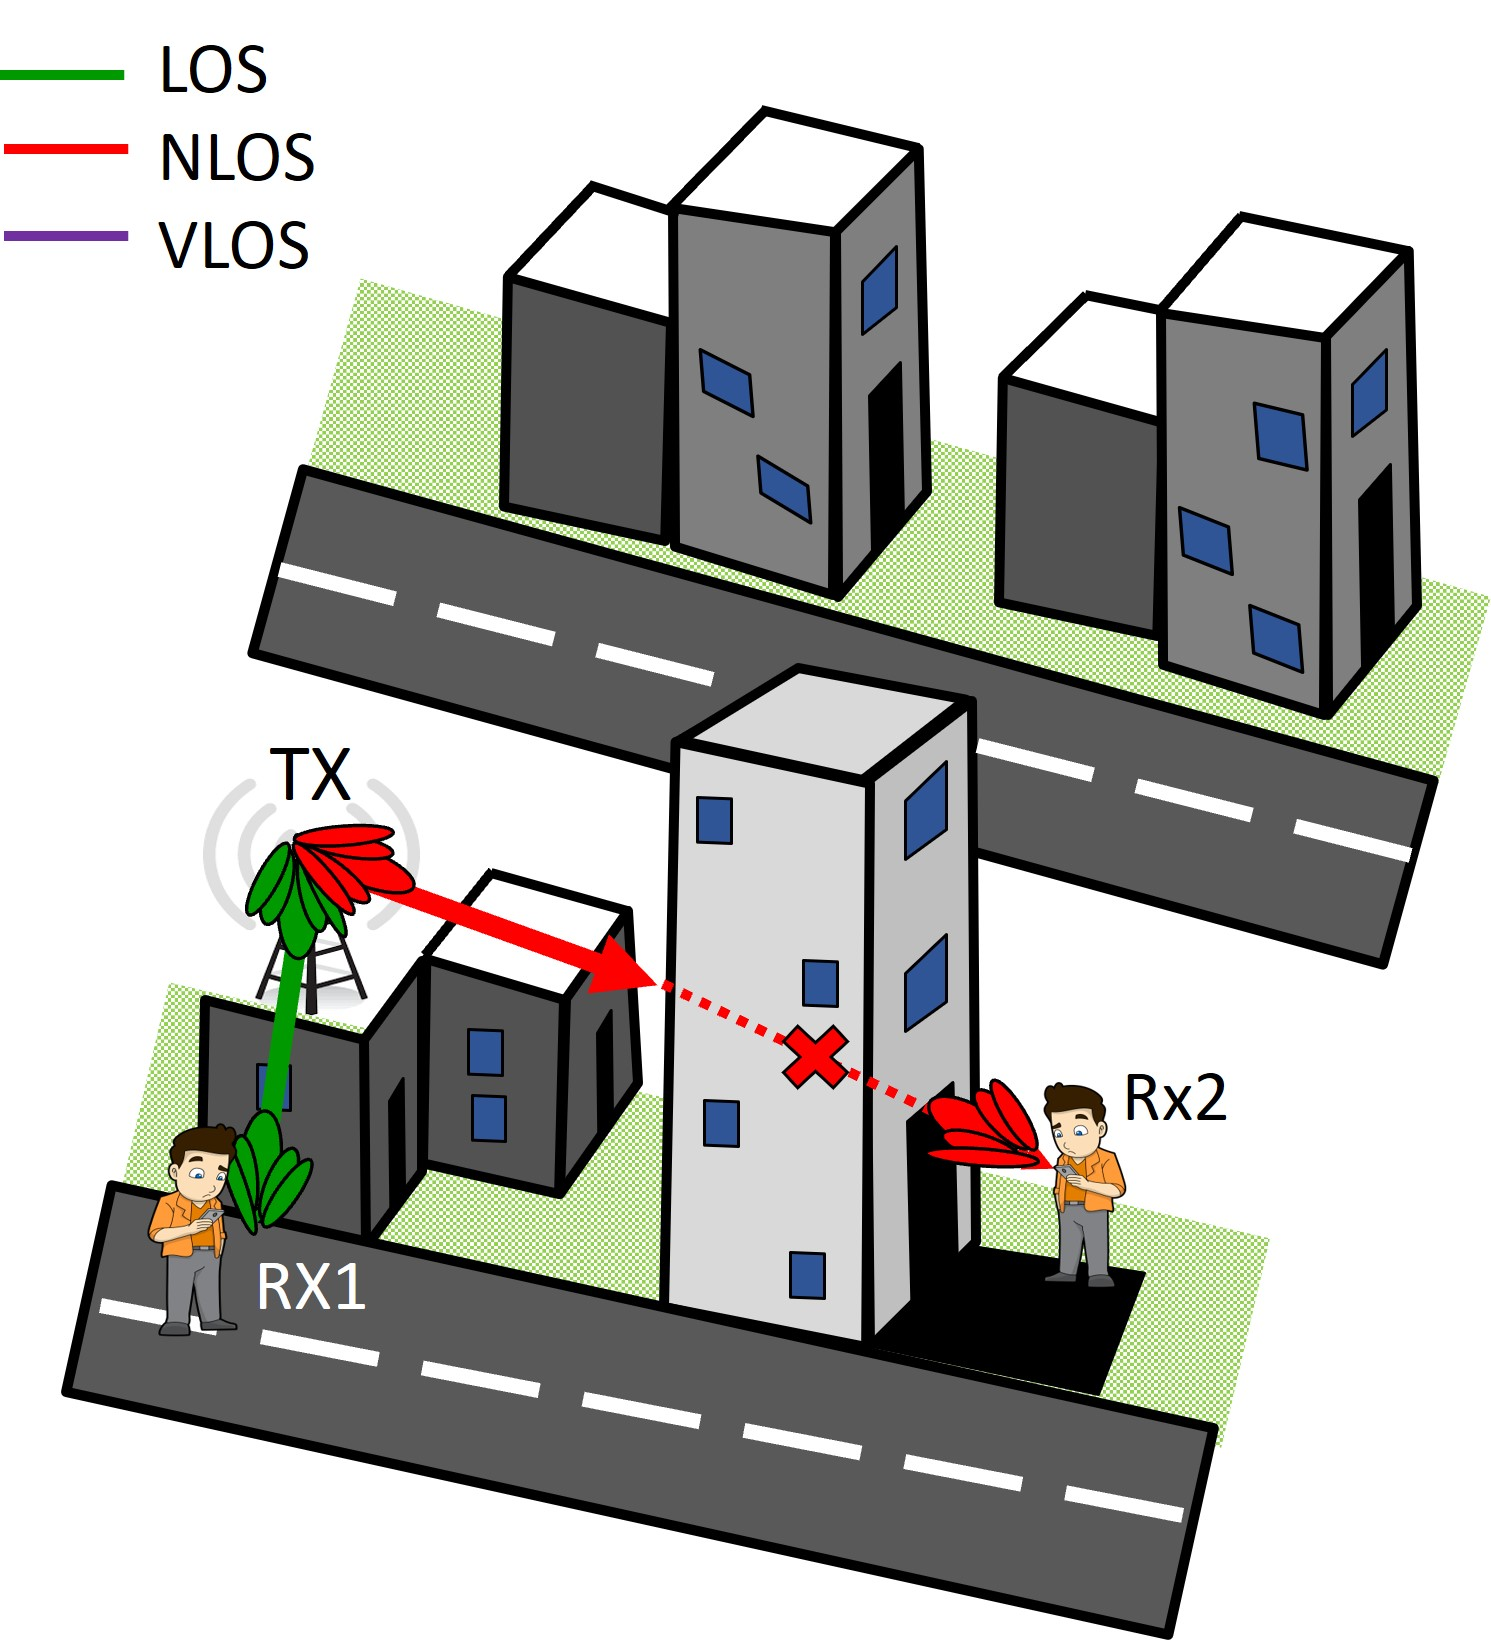
\includegraphics[width=0.45\linewidth]{images/Section 1 Images/Tx_Rx}
		\label{fig:Tx_Rx}
	}
	\hfill
	\subfloat[Future metasurface-enhanced mmWave networks can provide good connectivity in the NLOS regions by illuminating shadow regions using smart reflection behavior.]{
		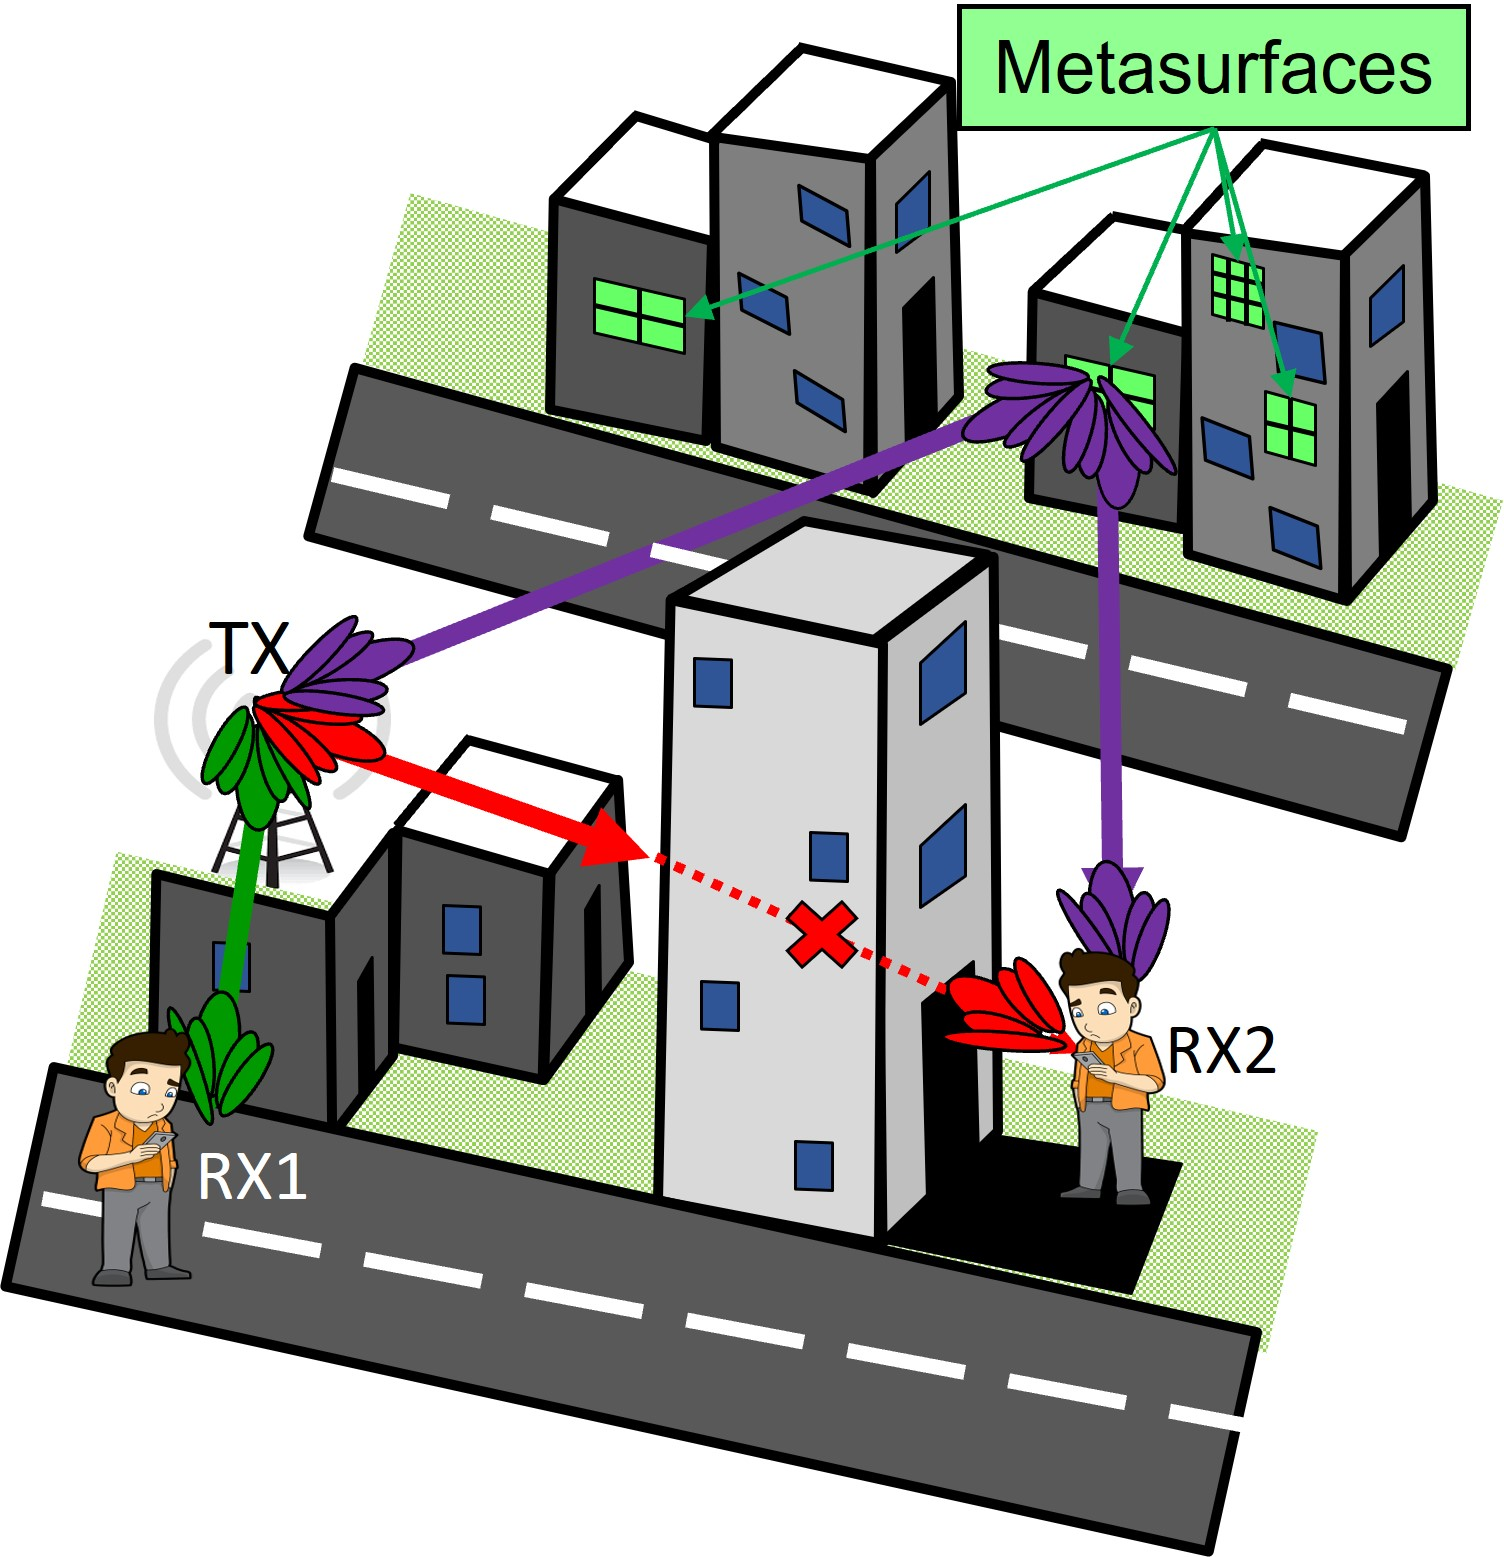
\includegraphics[width=0.45\linewidth]{images/Section 1 Images/Tx-Rx_Meta}
		\label{fig:Tx-Rx_Meta}
	}
	\caption[mmWave communication links from the transmitter (TX) to two differently positioned receivers (RXs): (a) RX1 in \ac{LOS} has a good connection, whereas RX2 in \ac{NLOS} cannot connect to the network. In (b) we illustrate how a metasurface that is mounted in the vicinity of the transceivers provides \ac{VLOS} connectivity to the \ac{NLOS} RX.]{mmWave communication links from the transmitter (TX) to two differently positioned receivers (RXs): (a) RX1 in \ac{LOS} has a good connection, whereas RX2 in \ac{NLOS} cannot connect to the network. In (b) we illustrate how a metasurface that is mounted in the vicinity of the transceivers provides \ac{VLOS} connectivity to the \ac{NLOS} RX.}
	\label{fig:Tx_RX}
\end{figure}
\ac{IRS} is a current hot topic in 6G research, primarily explored for its high flexibility by allowing dynamic control of reflected electromagnetic waves \cite{IRSdesignandapp, Shen2020ModelingAA, wu2019towards}. However, there are drawbacks to high energy consumption and active electronic components' complexity associated with \ac{IRS}. These challenges are not expected for the passive reflectors such as \ac{HELIOS} \cite{Helios}, making them the primary focus of this work.

In contrast to relying merely on simulations like current work, developing a HELIOS channel model or reflection model becomes critical since it provides a systematic analytical framework based on \ac{RCS} concepts \cite{Balanis, Kerr1989PropagationOS}. While simulation-based methods provide useful insights, an analytical model not only speeds up the computation, but it also enables a more rapid design and evaluation of passive reflector applications in urban communication networks. To demonstrate this practicality, we conduct a detailed analytical case study using HELIOS reflectors and compare them to \ac{IRS}s.

The remainder of this thesis is structured as follows. Sec. 2 of this master thesis introduces 5G mmWave communication before diving into the 6G metasurface concepts. Particularly, we introduce selected \ac{IRS} channel models and point out the lack of such for the recently proposed \ac{HELIOS} reflectors. Sec. 3 derives the analytical model of the bistatic RCS of \ac{HELIOS} reflectors and compares the arising reflection patterns to EM simulations. Sec. 4 assess the computing times before exploring our model in the context of an urban network scenario. There, we use it to optimize the connectivity and, at last, we directly compare \ac{IRS} and \ac{HELIOS} performance. Sec. 5 concludes this work by summarizing the key contributions and a brief outlook on future research.
%In the never-ending quest of wireless communication technology advancement, millimeter-wave (mmWave) frequencies have emerged, offering data speeds and network capacity. The basic qualities of mmWave, i.e., shorter wavelengths, make it a great choice for meeting the ever-increasing need for high-speed and high-capacity networks \cite{Intro1, ericsson6g, nokia6g}. However, the incorporation of mmWave into communication networks introduces high path loss due to obstructions, including greater atmospheric absorption and lower coverage \cite{6GWireless, 8373698}. As we look to the future, the transition to 6G seems inevitable. Beyond the capabilities of mmWave, 6G adds new concepts such as Smart Radio Environments (SREs) to improve network performance \cite{CNI}. SREs use intelligent components, in recent years, research into metasurfaces has received a lot of interest in the fields of wireless communications and radar technology. Metasurfaces, known for their capacity to precisely modify electromagnetic waves, have emerged as critical components in signal propagation. The two kinds of metasurfaces: Reconfigurable Intelligent Surfaces (RIS) and passive reflectors, interests us. Notably, the emphasis has switched from active to passive reflectors, representing a paradigm shift in research and development. These passive reflectors use the notion of altering signal reflections to improve coverage, and increase network efficiency by taking advantage of metasurfaces' natural benefits while reducing complexity and energy usage \cite{en14248219, LiSinghSievenpiper, FangLiChenSunXiaoHeZhou}.\\
%In light of this paradigm change, this thesis digs into the complexities of passive reflectors, proposing a complete methodology to optimize and expedite the use of these reflecting surfaces while also shining light on its distinguishing features and usefulness in modern communication systems. Unlike most simulation-based techniques, our work presents an analytical model based on Radar Cross-Section (RCS) principles that aims to speed up computations without sacrificing precision, opening the path for real-time applications in urban communication networks.\\

%We deploy the passive reflector in a simulated urban situation to validate our analytical model in practice \cite{Helios}. This implementation is intended to evaluate the analytical model's performance and efficacy in a dynamic and difficult context. In this thesis work, we go deeper into the theoretical underpinnings, design principles, and empirical validations, providing a holistic examination of passive reflectors' revolutionary potential in the mmWave and 6G landscapes.\\
%\Cref{fig:Tx_Rx} displays a standard communication scenario similar to a typical 5G network with transmitter (Tx) and two receivers (Rx1 and Rx2) where Rx1 has a Line-of-Sight (LOS) path and Rx2 encounters a Non-Line-of-Sight (NLOS) path to the Tx, resulting in path losses designated as $PL_{Tx. Rx1}$, and $PL_{Tx. Rx2}$, respectively, in \si{\decibel}.
%\Cref{fig:Tx-Rx_Meta} depicts a transformational perspective in the context of 6G communication, proposing a metasurface to handle NLOS circumstances. Notably, when there is an NLOS path between Tx and Rx2, a virtual LOS connection is constructed by including a metasurface mounted on the building. $PL_1$, and $PL_2$ indicate the path losses associated here as depicted. Unlike classic NLOS scenarios, the metasurface presents a unique signal attenuation mitigation technique, which has the potential to improve communication reliability and performance.\\
%\Cref{cha:Background} of our thesis begins by explaining the motives for harnessing mmWave communication and investigating solutions such as SREs and metasurfaces. We introduce known IRS models and compare them with the novel notion of HELIOS passive reflectors. \Cref{Simulation and Analytical Modeling of HELIOS Reflectors} focuses on the derivation of our analytical model for the HELIOS model's reflection pattern, using bistatic RCS principles and comparing the findings to EM simulations. In \Cref{Performance Evaluation and Case Study}, we undertake a complete performance evaluation, comparing our analytical model's computational time to EM simulations. Expanding our analysis, we build an urban environment, anticipate communication channel models, and aim to optimize the model by changing the geometry and reflector position. \Cref{Conclusion} concludes this work by summarizing our accomplishments and laying the groundwork for future research by identifying potential areas for investigation and improvement.
